\documentclass[a4paper]{article}

%% Language and font encodings
\usepackage[english]{babel}
\usepackage[utf8x]{inputenc}
\usepackage[T1]{fontenc}
\usepackage{datetime}
\newdate{date}{10}{03}{2017}
\newcommand\tab[1][1cm]{\hspace*{#1}}
\usepackage{amsfonts}

%% Sets page size and margins
\usepackage[a4paper,top=3cm,bottom=2cm,left=3cm,right=3cm,marginparwidth=1.75cm]{geometry}

%% Useful packages
\usepackage{amsmath}
\usepackage{graphicx}
\usepackage[colorinlistoftodos]{todonotes}
\usepackage[colorlinks=true, allcolors=blue]{hyperref}
\usepackage{enumitem}   



\title{Tutorial 5}
\date{\displaydate{date}}
\begin{document}
\maketitle

\begin{enumerate}
\item For $n \geq 2$, let $G = (V, E)$ be the loop-free undirected graph, where $V$ is the set of binary strings of length $n$, and $E = \{(v, w)| v, w \in V$ and v, w differ in (exactly) two
positions$\}$. Find $\kappa (G)$. \\

Solution: \\
It can be shown that such a graph will always have two components, independent of $n$. All the strings with an even number of 1's in the string will belong to one component while those with an odd number of 1's in the string will belong to the other component. \\
Let $C_e$ be the component with strings having even number of 1's. \\
We know that the string $0^n = s_0 \in C_e$. \\
Given any string $s_i \in C_e$, we obtain string $s_{i1}$ by flipping the first 2 occurrences of 1's in $s_i$ to 0s. Also, we see that such a string $s_{i1} \in C_e$ and $(s_i, s_{i1}) \in E$, i.e there is edge between $s_i$ and $s_{i1}$. \\ 
Similarly, we can obtain a sequence of strings $s_{i2}, s_{i3}, \dots s_0$. \\
Thus, we proved that every string with even number of 1's has a path to the string $s_0$.\\

Let $C_o$ be the component with all those strings having an odd number of 1's. \\
We know that the string $10^{n-1} = s_1 \in C_e$. \\
With a similar argument as stated previously, we see that every string $s_j \in C_o \ni '$ the first bit of $s_j$ is 1, we see that $s_j$ has a path to $s_1$. \\
For all those string $s_k \in C_o \ni '$ first bit is 0, we obtain a string $s_{k'}$ by changing the first bit to 1 and the first occurrence of 1 to 0. Then the previous argument can be made to say that $s_k$ and $s_1$ are connected. \\
Additionally we note that no string in $C_o$ is connected to a string in $C_e$ as change in 2 bits in the string would ensure that the parity of 1's in the string remains the same.\\

\begin{center}
------------ X ------------
\end{center} 

\item The department store wants to set up a security system where
(plainclothes) guards are placed at certain cashier locations so
that each cashier either has a guard at his or her location or is
only one aisle away from a cashier who has a guard. How should they decide what is
the smallest number of guards needed? Design a solution for an example scenario.\\

Solution\\
We can model the problem as a graph such that each cash counter is a node and those cashiers who are an aisle away have an edge between the corresponding nodes.\\
For example, the following would be the floor plan of some department store:
\begin{figure}[h]
\centering
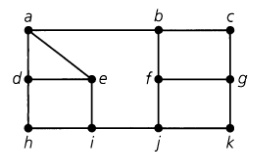
\includegraphics[scale=0.5]{dept.png}
\end{figure}
In this case, we can see that 3 guards at $a, i, g$ would suffice.\\
Also we can conclude that nothing lesser than 3 would work as the maximum degree of nodes in the graph is 3.\\

\begin{center}
------------ X ------------
\end{center} 

\item Define a $wheel$ graph $W_n$.
\begin{enumerate}
\item Determine how many cycles of length 4 there are in each of $W_3, W_4, W_5$?
\item Given $n \in Z^+$ and $n \geq 3$, how many
cycles of length 4 are there in $W_n$?
\item How many cycles in $W_n$ have length $n$?
\end{enumerate} 

Solution: \\
In general, if $n \in Z^+$ and $n\geq 3$, then the wheel with $n$
spokes is the graph made up of a cycle of length $n$ together
with an additional vertex that is adjacent to the $n$ vertices
of the cycle. The graph is denoted by $W_n$.\\

$W_3, W_4, W_5$ have 3, 5, 5 cycles of length four respectively.\\

For any wheel such that $n \geq 4$, we see that each cycle of length 4 must include the vertex at the center ($v_{n+1}$). \\
For every vertex $v_i \ni ' i \neq (n+1)$, it is associated with a cycle on $v_{i+2}$ and another with $v_{i-1}$. This is because $v_i$ on a cycle with any other vertex would lead to increase in the path length. Thus there are $n$ four length cycles in $W_n$, where $n \geq 5$. \\

Similarly, we can see that there are $n+1$ cycles of length $n$. There are $n$ cycles including the center vertex and 1 excluding it.
\\

\begin{center}
------------ X ------------
\end{center}  

\item If $G = (V, E)$ is an undirected graph, how many spanning
subgraphs of $G$ are also induced subgraphs?\\
Solution: Only $G$ itself. 
\begin{center}
------------ X ------------
\end{center} 

\item Let $G = (V, E)$ be an undirected graph, where $|V| \geq 2$. If
every induced subgraph of $G$ is connected, can we identify the
graph $G$?\\
Solution : $G$ would be the complete graph $K_n$, since we can conclude that every pair of vertices must be connected when we choose the induced subgraph on these two vertices.\\
\begin{center}
------------ X ------------
\end{center} 

\item Let $m,n \in Z^+$ with $m <n$. How many paths of length $m$ are there in the complete graph $K_n$? \\
Solution: \\
$\frac{1}{2} \{n(n-1)\dots (n-m)\}$\\
This is because we can have a $n$ length path between any two pair of nodes since the given graph is complete.\\
There are $n$ choices for the first node, $n-1$ choices for the $2^{nd}$ , and so on until the $m+1^{th}$ node. \\
We divide by two to ensure we count the path between nodes $x$ and $y$ only once. 
\begin{center}
------------ X ------------
\end{center} 





\item Let $G$ be an undirected graph with 
$n$ vertices. If $G$ is
isomorphic to its own complement $\overline{G}$, how many edges must
$G$ have? Give an example of such a graph.\\
Solution:\\

Total number of edges in a graph is $n \choose 2$.\\
If $G$ is isomorphic to $\overline{G}$, then both have the same number of edges = $\frac{n(n-1)}{4}$
\begin{center}
------------ X ------------
\end{center}



\item If $G$ is a self-complementary graph on $n$ vertices, where
$n > 1$, prove that $n = 4k$ or $n = 4k + 1$, for some $k \in Z^+$.\\
Solution: \\
From the previous question, we can conclude that $\frac{n(n-1)}{4}$ is an integer. Also, we see that either of $n$ or $n-1$ is odd.\\
Therefore, we conclude either $4|n$ or $4|n-1$. \\
Thus, $n \equiv 4k$ or $n \equiv 4k+1$
\begin{center}
------------ X ------------
\end{center}

\item
\begin{enumerate}
\item Find a graph $G$ where both $G$ and $\overline{G}$ are connected.\\
Solution:\\
\begin{figure}[h]
\centering
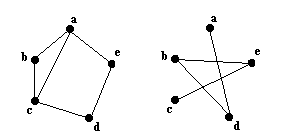
\includegraphics[scale=0.5]{complement.png}
\end{figure}

\item If $G$ is a graph on $n$ vertices, for $n \geq 2$, and $G$ is not connected, prove that $\overline{G}$ is connected.\\
Solution: \\
Since $G$ is not connected, there must be at least 2 components in the graph $C_1,C_2$. For every node $x \in C_1$ and $y \in C_2$, 
$(x,y) \in \overline{G}$. \\
For every pair of nodes $x_1,x_2 \in C_1$, if the pair were connected by an edge in $G$, now there is a two length path in $\overline{G} \rightarrow x_1,y,x_2$. Else they are connected by an edge in $\overline{G}$. \\
 
\end{enumerate}


\end{enumerate}
\end{document}
